\documentclass[12pt,a4paper]{article}
\usepackage[legalpaper, portrait, margin=2cm]{geometry}
\usepackage[export]{adjustbox}
\usepackage{fancyhdr}
\usepackage{graphicx}
\usepackage{hyperref}
\usepackage{listings}
\usepackage{xcolor}
\usepackage{setspace}

\graphicspath{ {./docs/} }

\hypersetup{
	citecolor=blue,
	colorlinks=true,
	filecolor=magenta,
	linkcolor=blue,
	pdfpagemode=FullScreen,
	pdftitle={Homework I - Group 67},
	urlcolor=blue,
}

\definecolor{codegreen}{rgb}{0,0.6,0}
\definecolor{codegray}{rgb}{0.5,0.5,0.5}
\definecolor{codepurple}{rgb}{0.58,0,0.82}
\definecolor{backcolour}{rgb}{0.95,0.95,0.92}

\lstdefinestyle{Python}{
    basicstyle=\ttfamily\footnotesize,
    breakatwhitespace=false,
    breaklines=true,
    captionpos=b,
    commentstyle=\color{codegreen},
    keepspaces=true,
    keywordstyle=\color{magenta},
    numbers=left,
    numbersep=5pt,
    numberstyle=\tiny\color{codegray},
    showspaces=false,
    showstringspaces=false,
    showtabs=false,
    stringstyle=\color{codepurple},
    tabsize=2
}

\lstset{style=Python}

\pagestyle{fancy}
\fancyhf{}
\rhead{Grupo \textbf{67}}
\lhead{Aprendizagem 2022/23 - Homework I}
\cfoot{Luís Câmara (99099) e Pedro Lobo (99115)}

\renewcommand{\familydefault}{CambriaMath}
\renewcommand{\thesection}{\Roman{section}}
\renewcommand{\thesubsection}{\arabic{subsection}}

\begin{document}

\section{Pen-and-paper}
\begin{enumerate}
	\item
	      \hfill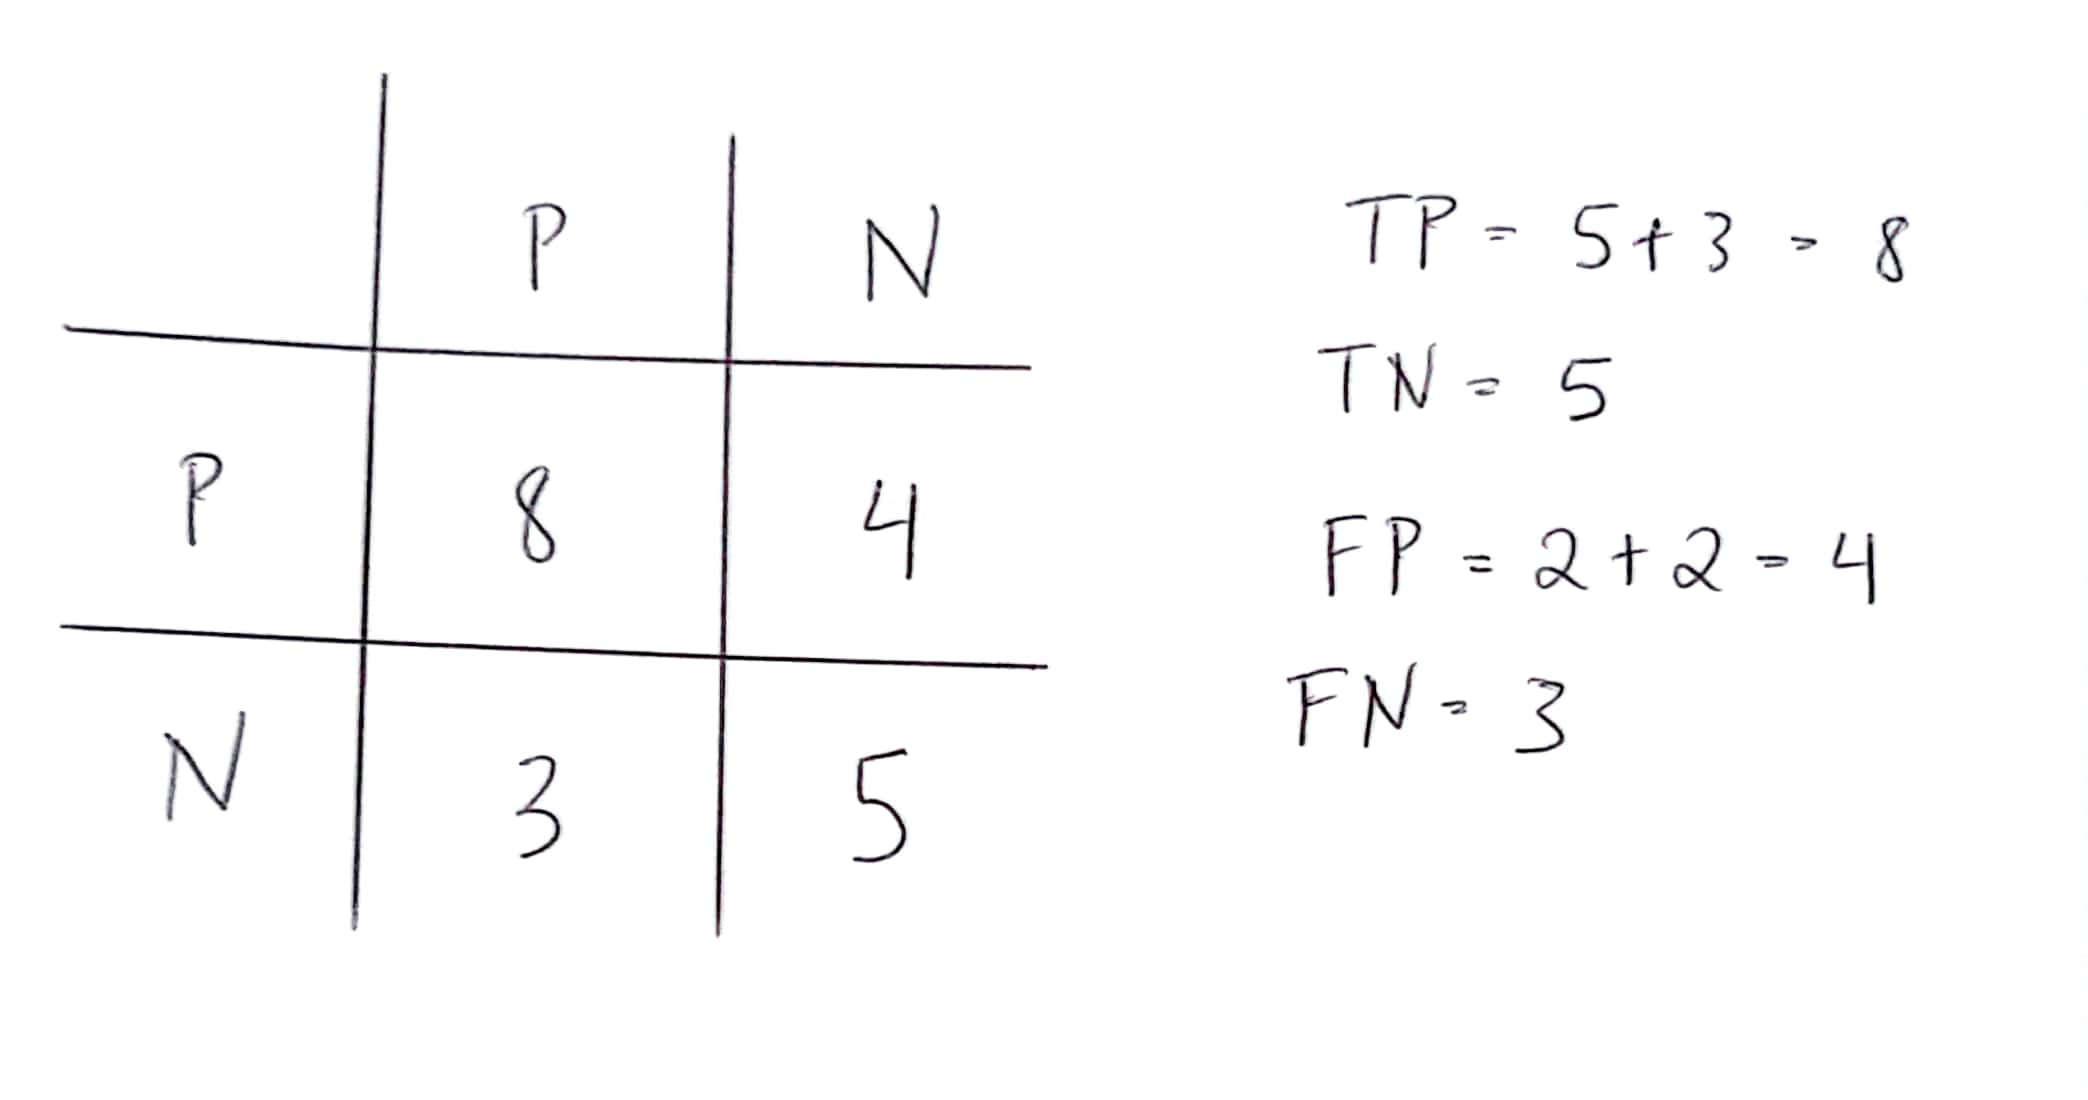
\includegraphics[scale=0.13,valign=t]{1.jpg}\hspace*{\fill}

	      \vspace{40px}

	\item
	      \hfill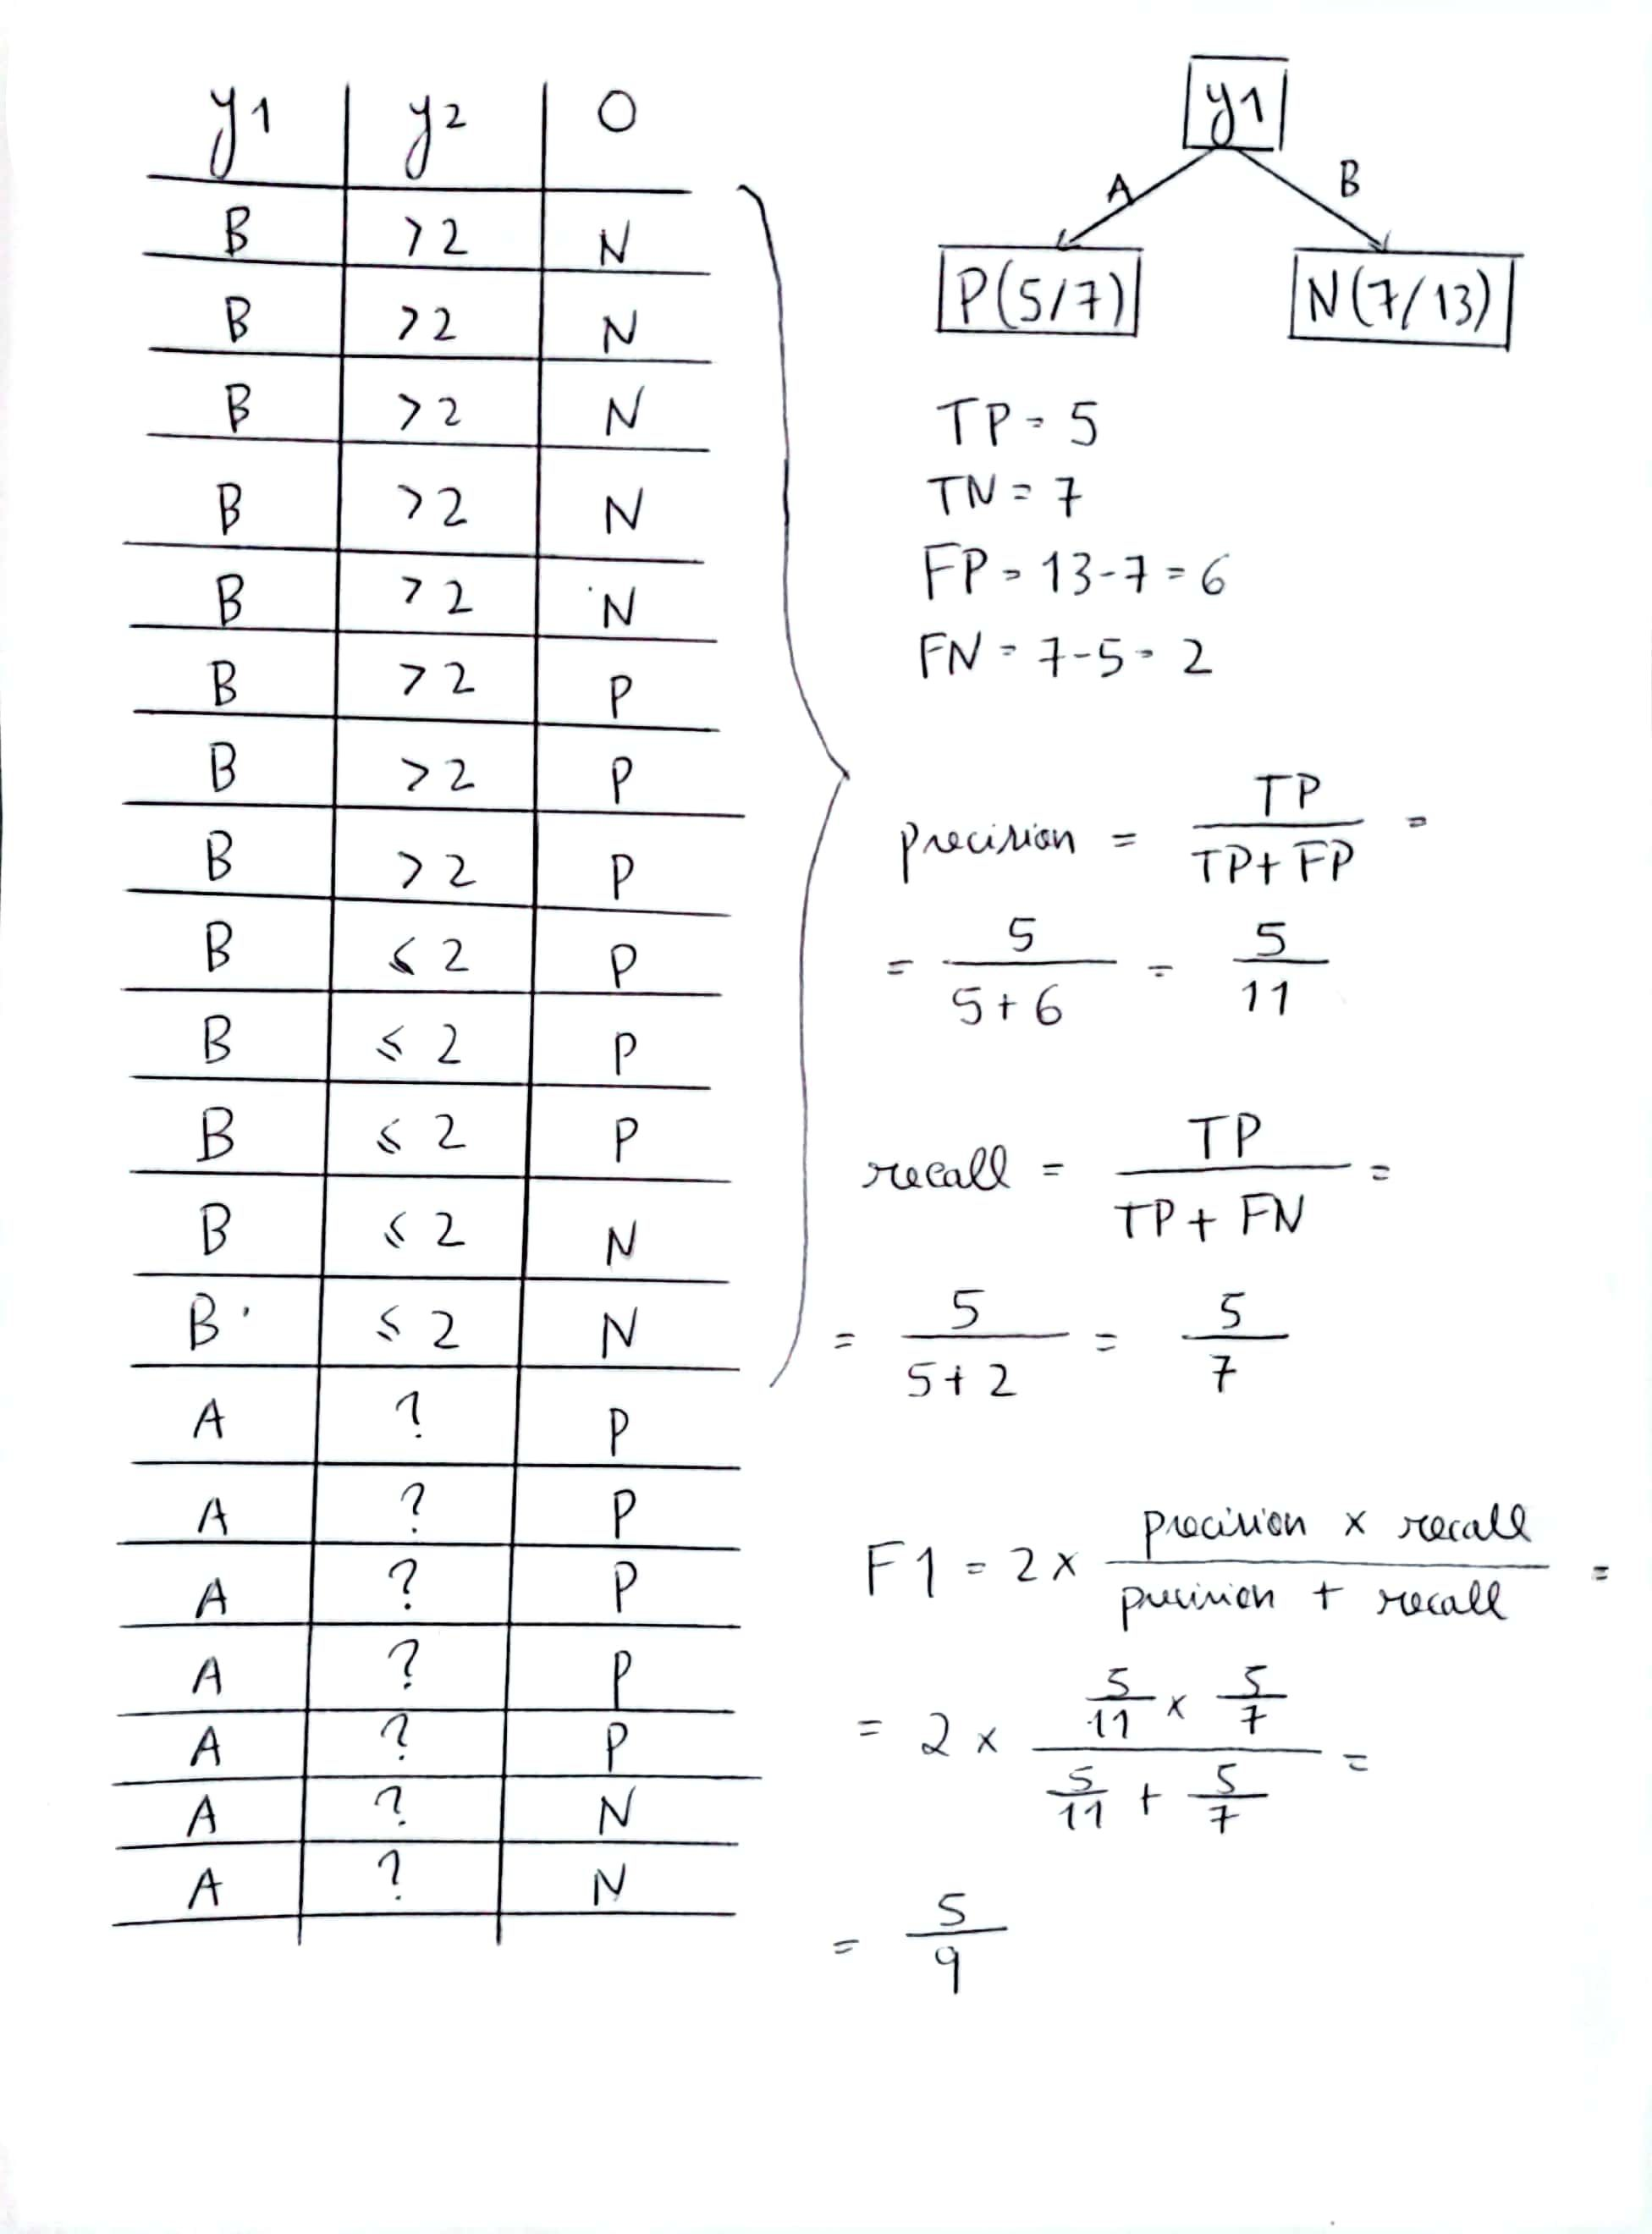
\includegraphics[scale=0.2,valign=t]{2}\hspace*{\fill}

	\item
	      \hfill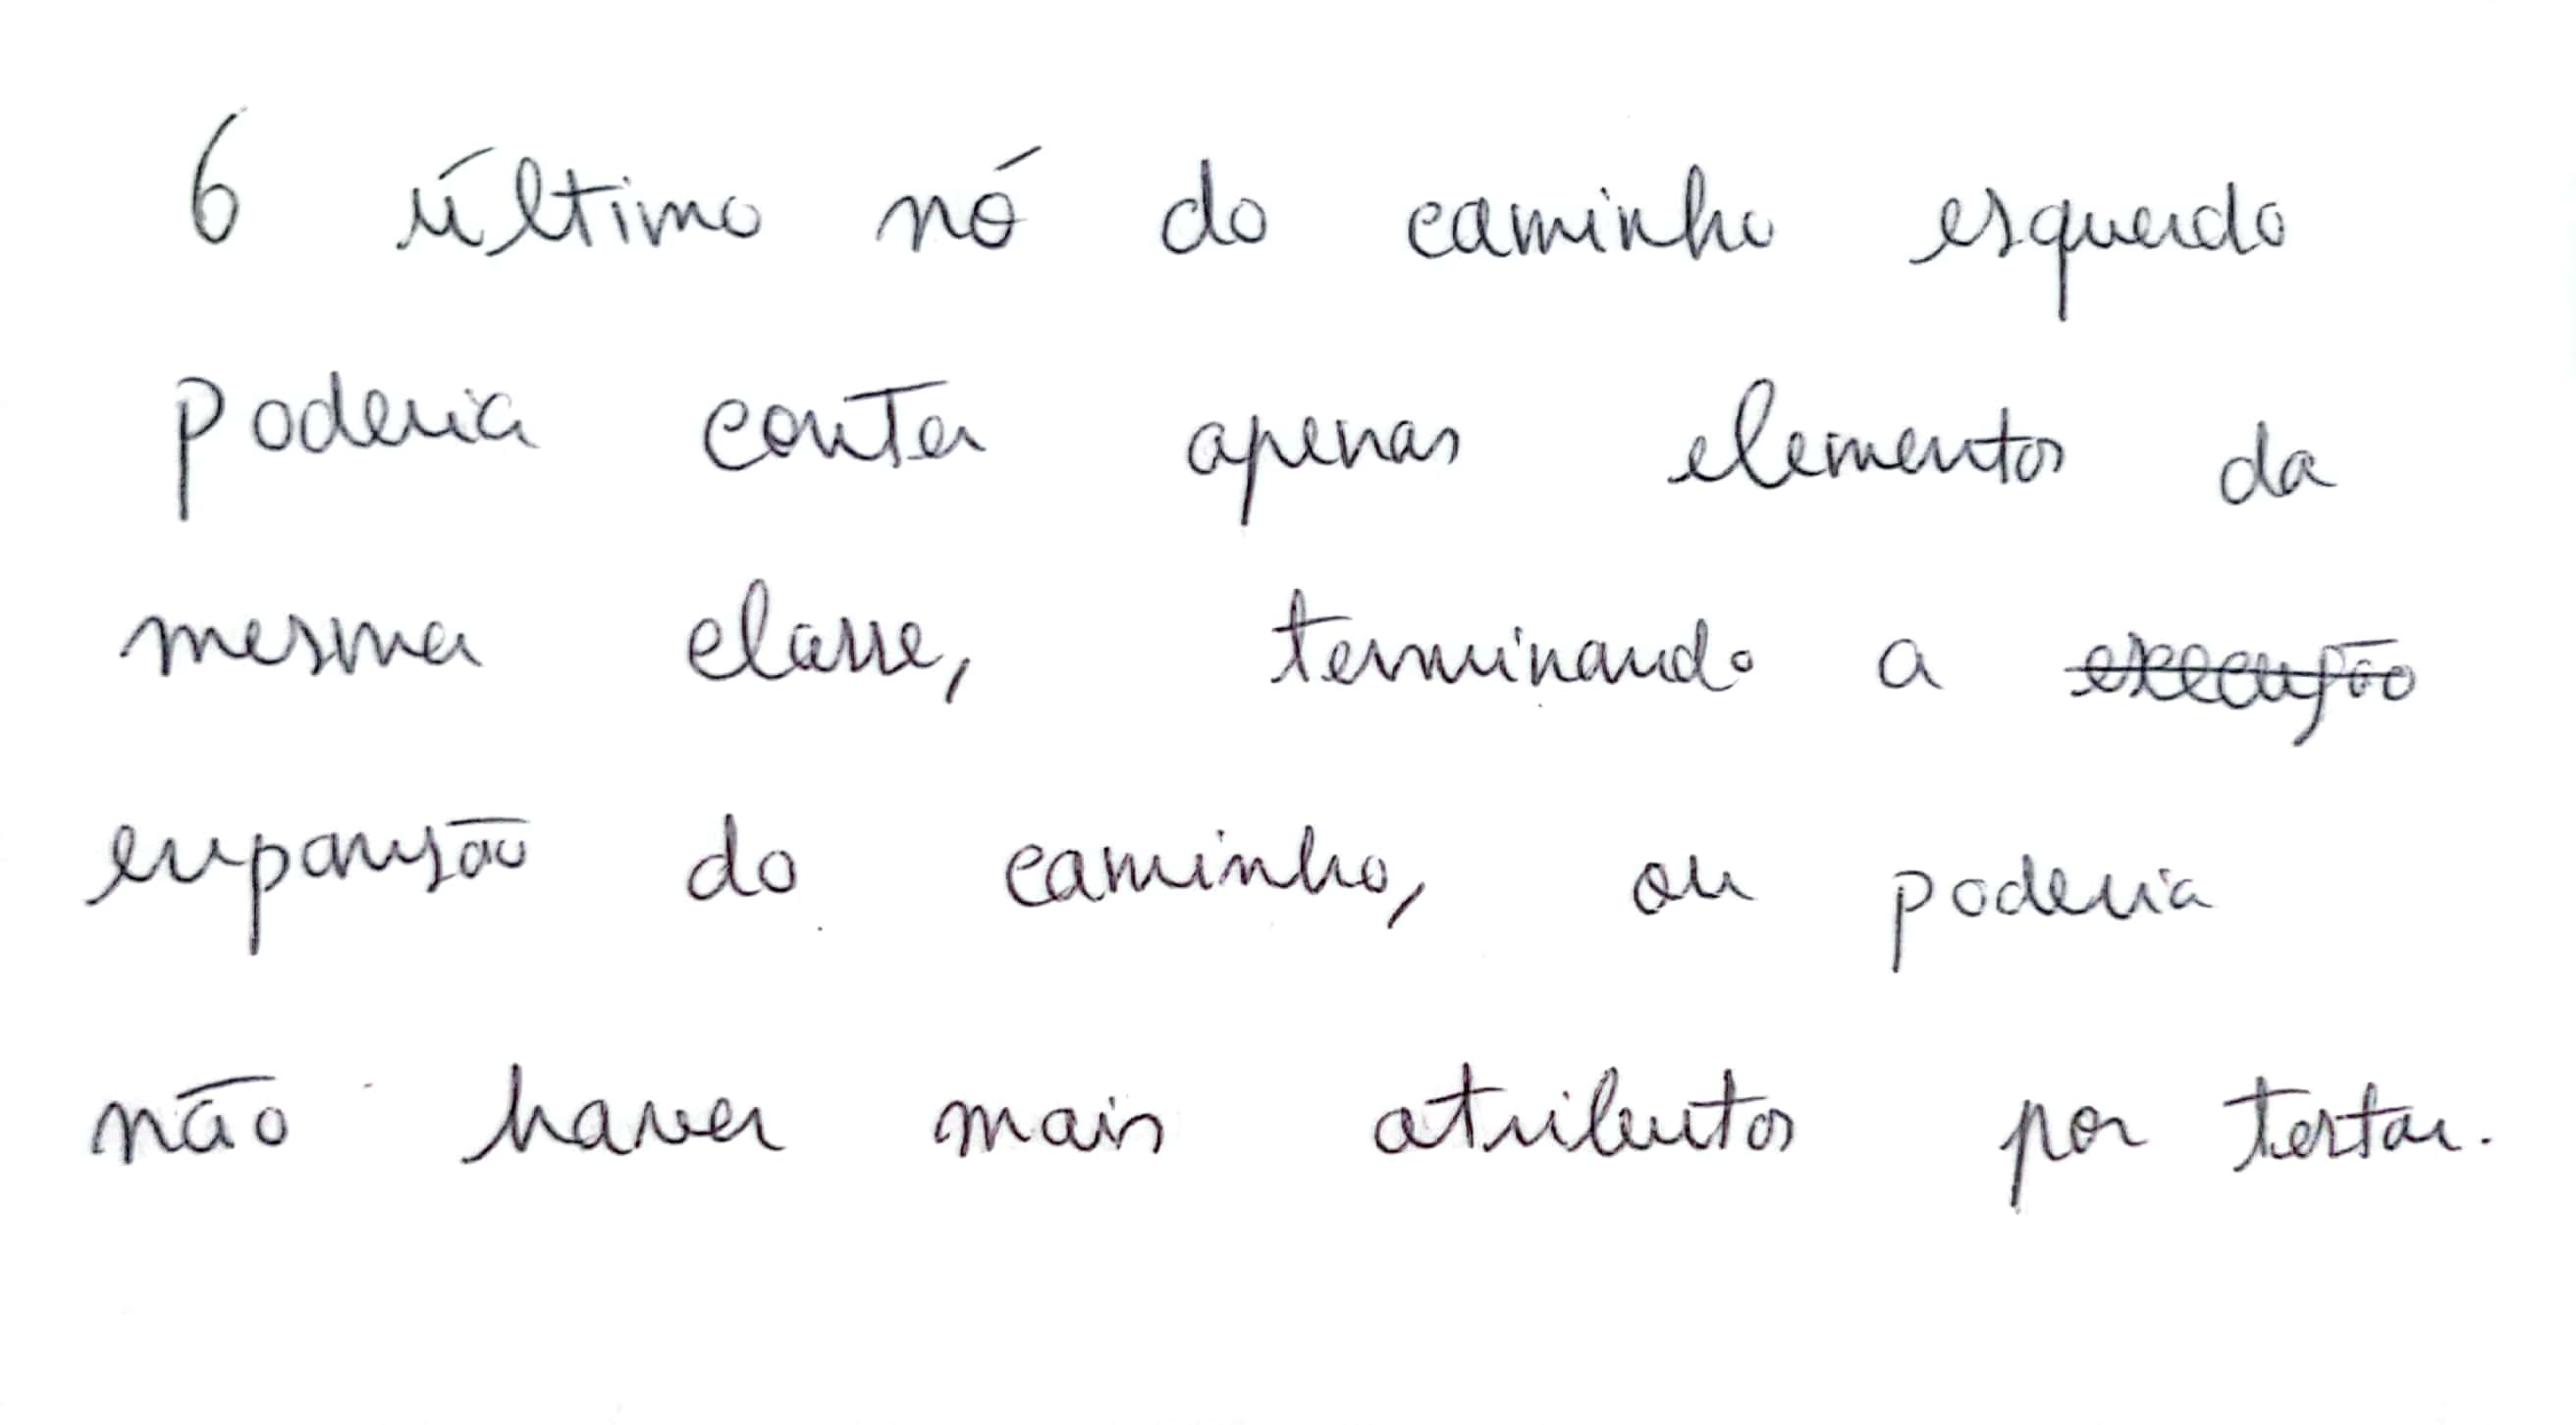
\includegraphics[scale=0.15,valign=t]{3}\hspace*{\fill}

	      \vspace{20px}

	\item
	      \hfill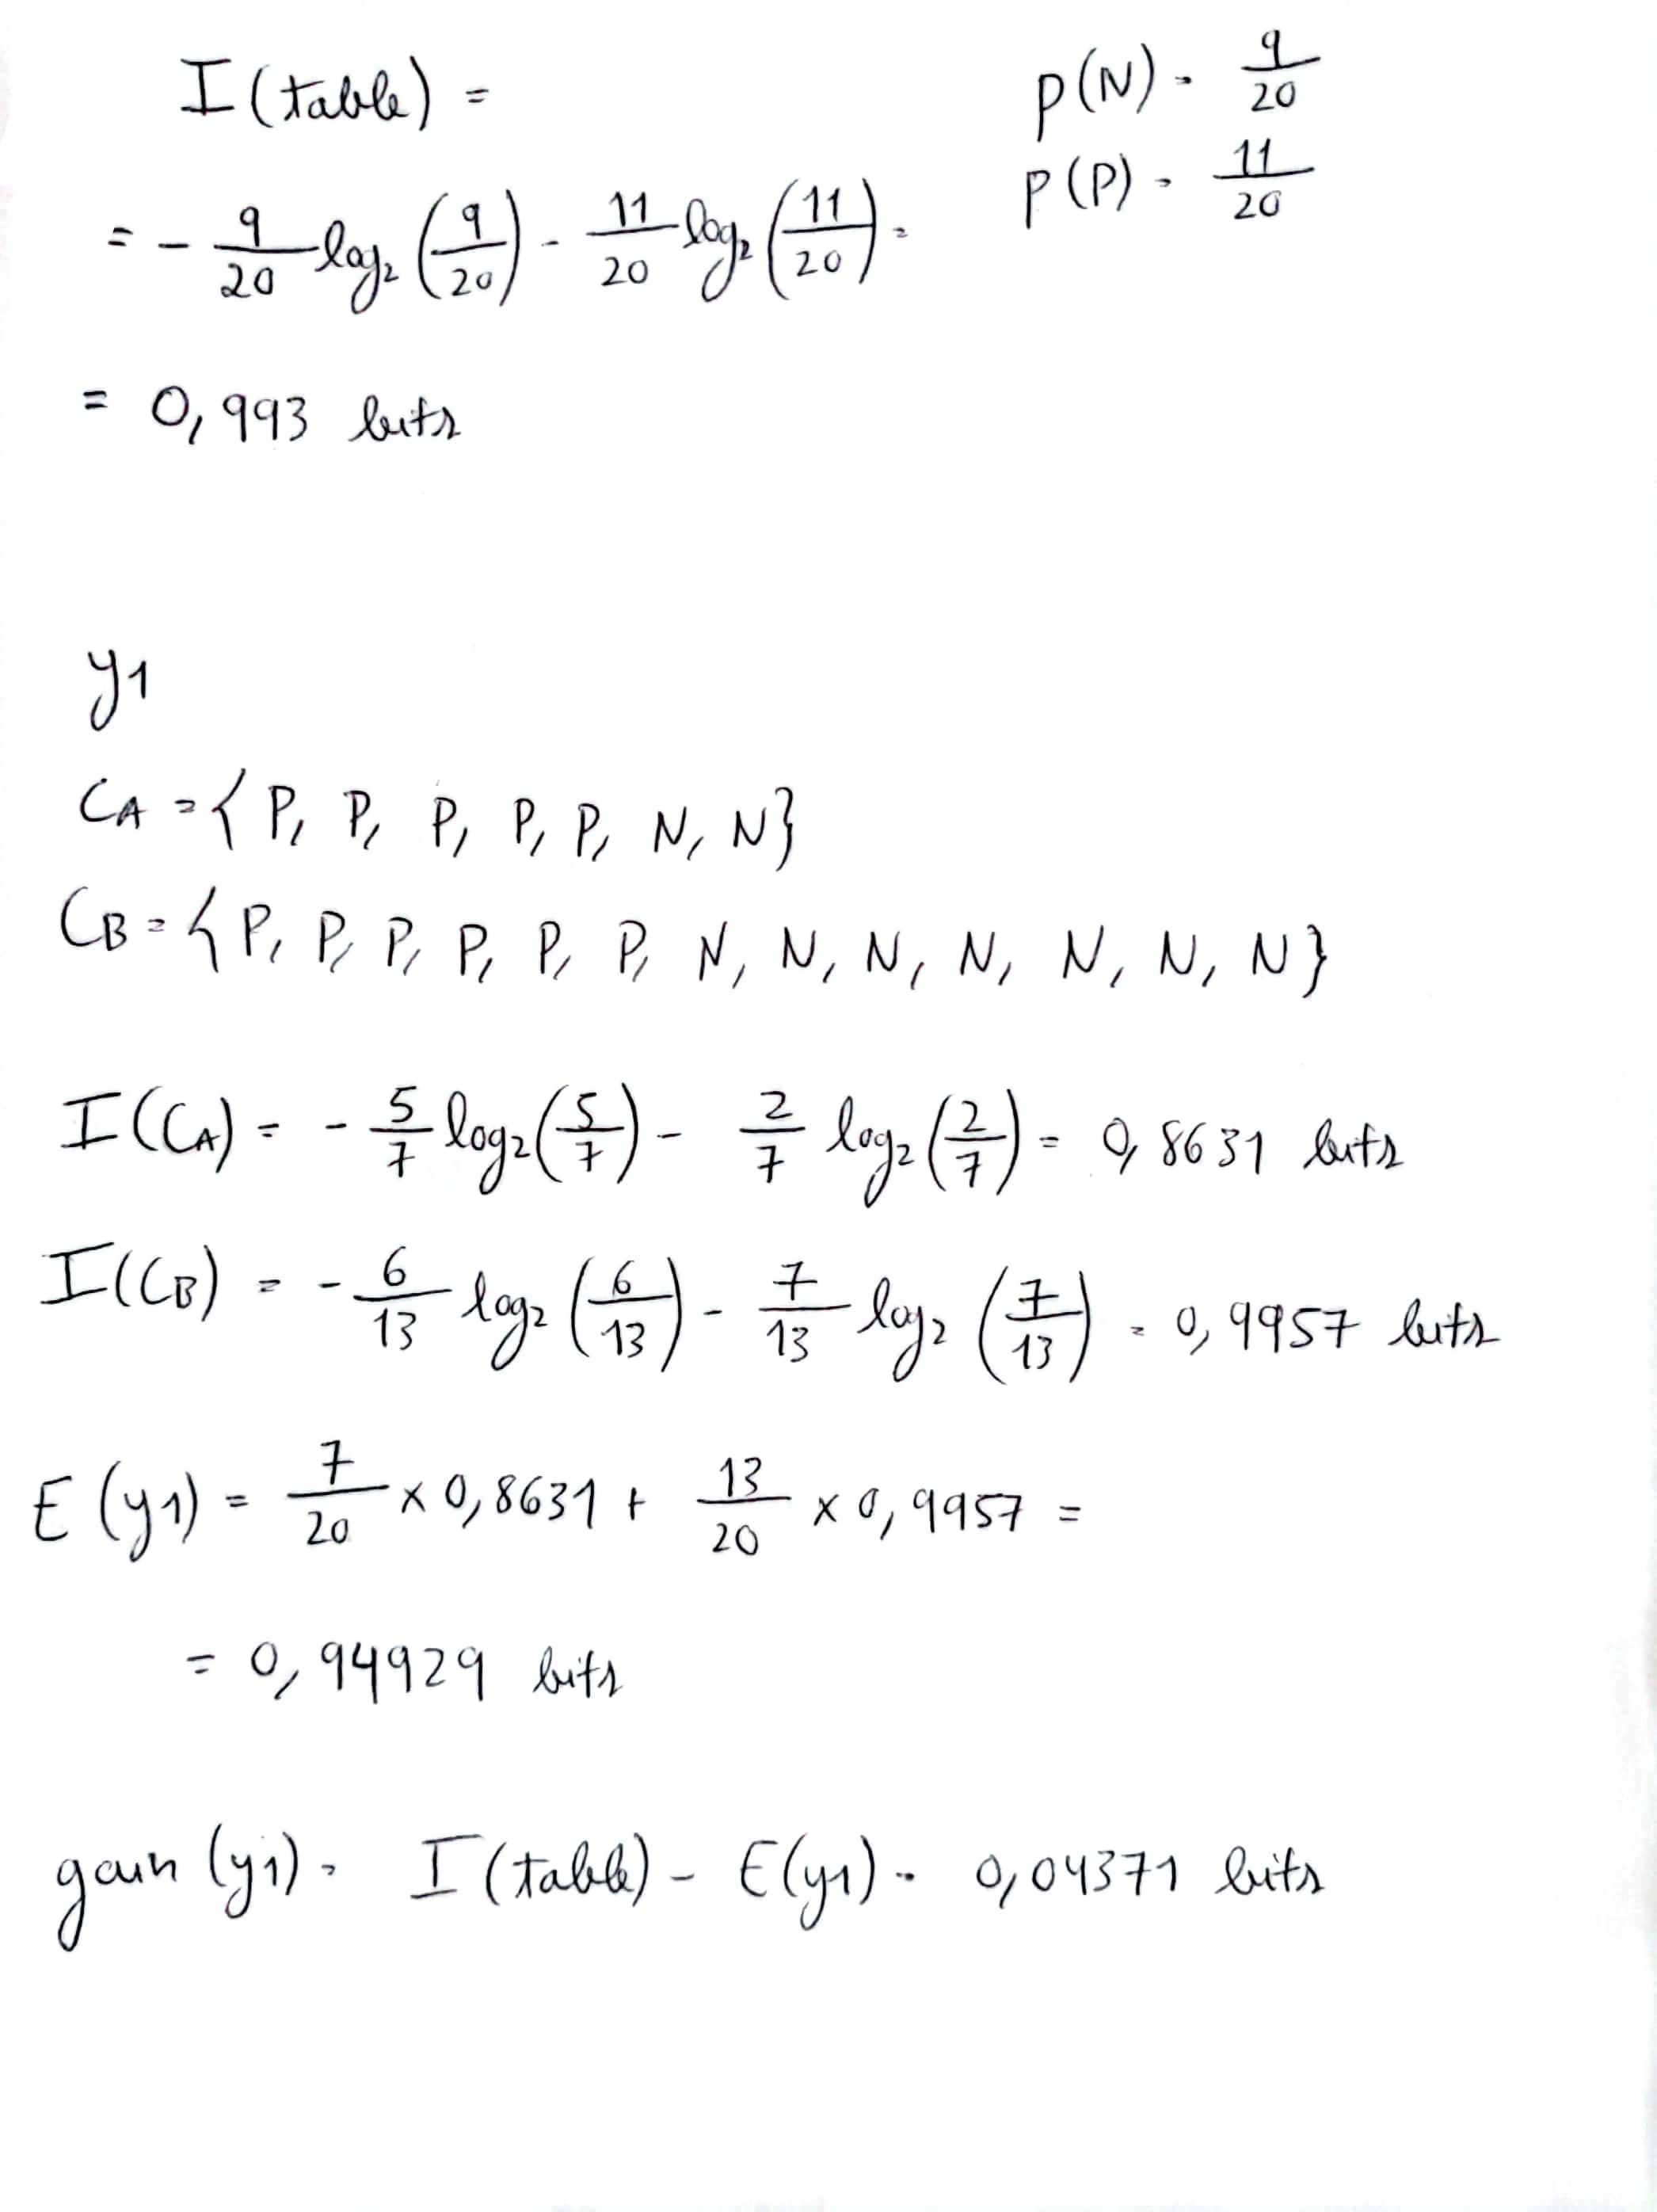
\includegraphics[scale=0.21,valign=t]{4}\hspace*{\fill}

\end{enumerate}

\pagebreak

\section{Programming}
\begin{enumerate}
	\item
	      \begin{center}
	      	\hfill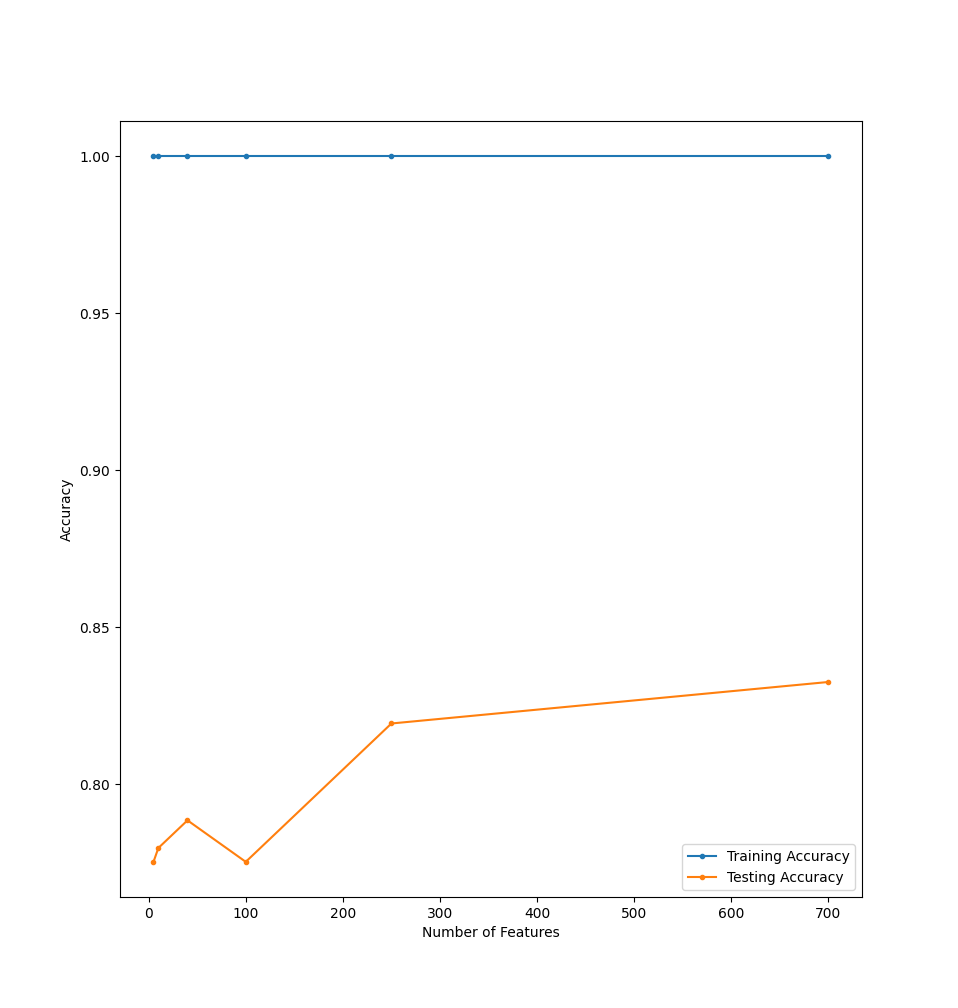
\includegraphics[scale=0.6,valign=t]{plot}\hspace*{\fill}
	      \end{center}

	      \vspace{20px}
	      \setstretch{1.5}

	\item
	      From the gathered results, we can conclude that there is a large
	      difference between the training accuracy and the testing accuracy.
	      The results show a training accuracy of 1, therefore, the model is
	      overfitting to the training set and doesn't generalize so nicely to
	      the testing set.

\end{enumerate}

\pagebreak

\section{Appendix}
\lstinputlisting[language=Python]{./src/code.py}

\end{document}
